\documentclass{article}
\usepackage[utf8]{inputenc}
\usepackage{tikz} %package for plots, graphics and functions

\title{For Loops}
\author{Arman Daneshdoost}
\date{March 2024}

\begin{document}
	\maketitle
		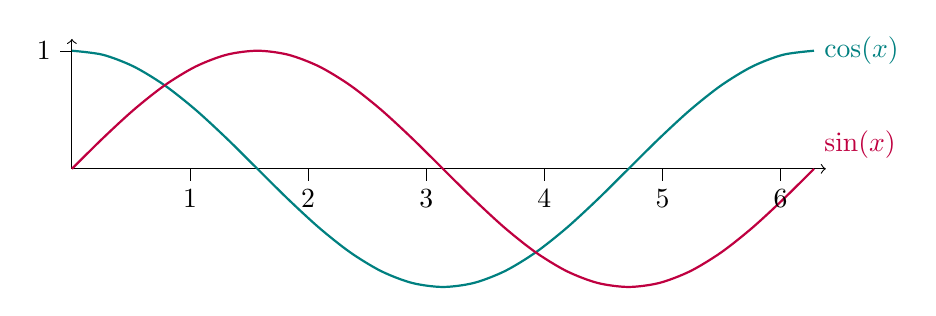
\begin{tikzpicture}[domain = 0:2*pi, scale=1.5]
		\draw [<->] (2*pi + 0.1, 0) -- (0, 0) -- (0, 1.1);
		\draw[smooth, teal, thick] plot (\x, {cos(\x r)})
		node[right]{$\cos(x)$};
		\draw[smooth, purple, thick] plot (\x, {sin(\x r)})
		node[above right]{$\sin(x)$};
		\foreach \x in {1,...,6}{
		\draw [ultra thin] (\x, 0) -- (\x, -0.1) node [below] {$\x$};}
		\draw [ultra thin] (0, 1) -- (-0.1, 1) node [left] {$1$};
		\end{tikzpicture}
\end{document}